% 电场
% 电场|库仑力|万有引力|点电荷|电磁学
\pentry{库仑定律\upref{ClbFrc}}

在经典电磁理论中, 电荷与电荷之间的作用力是通过场的作用产生的. 所以点电荷 $q_1$ 对另一个点电荷 $q_2$ 的库仑力可以理解为 $q_1$ 在其周围产生了电场对 $q_2$ 的作用(反之亦然).

注意在点电荷模型中, 我们假设一个点电荷产生的电场对其自身合力为 0. 另外, 我们一般不讨论点电荷所在位置处的电场强度, 我们可以说电场在该点处没有定义.

电场是可以叠加的, 当空间中有 $N$ 个点电荷, 空间中某点(除了这些电荷所在的点)处的电场等于每个点电荷在该点产生的电场之和. 注意这个求和是矢量相加.

在某个时刻, 空间中的电场是位置 $\bvec r$ 的矢量函数, 即任意一个 $\bvec r$ 对应一个唯一矢量 $\bvec E$. 我们把这个函数记为 $\bvec E(\bvec r)$. 当另一个点电荷处于这个电场中, 它就会受到电场力
\begin{equation}\label{Efield_eq1}
\bvec F(\bvec r) = q \bvec E(\bvec r)
\end{equation}
这个力也是位置的函数, 也就是一个力场\upref{V}.
 
\subsection{点电荷的电场}
现在我们可以用\autoref{Efield_eq1} 推出点电荷电场的表达式. $q_1$ 对 $q_2$ 的库仑力为(\autoref{ClbFrc_eq1}\upref{ClbFrc})
\begin{equation}\label{Efield_eq3}
\bvec F_{12} = q_2 \bvec E_1(\bvec r_2) = \frac{1}{4\pi\epsilon_0}\frac{q_1 q_2}{\abs{\bvec r_2 - \bvec r_1}^2} \uvec r_{12}
\end{equation}
其中 $\bvec E_1(\bvec r)$ 是 $q_1$ 单独产生的电场分布. 两边除以 $q_2$ 得
\begin{equation}
\bvec E_1(\bvec r_2) = \frac{1}{4\pi\epsilon_0}\frac{q_1}{\abs{\bvec r_2 - \bvec r_1}^2} \uvec r_{12}
\end{equation}

所以, 任意点位于 $\bvec r_i$ 处的点电荷 $q_i$ 产生的电场为
\begin{equation}\label{Efield_eq4}
\bvec E(\bvec r) = \frac{1}{4\pi\epsilon_0}\frac{q_i}{\abs{\bvec r - \bvec r_i}^2} \uvec R_i
\end{equation}
其中 $\uvec R_i = (\bvec r - \bvec r_i) / \abs{\bvec r - \bvec r_i}$ 是由 $\bvec r_i$ 指向 $\bvec r$ 的单位矢量. 由于电场可叠加, 空间中的 $N$ 个电荷产生的电场为
\begin{equation}\label{Efield_eq2}
\bvec E(\bvec r) = \frac{1}{4\pi\epsilon_0} \sum_{i=1}^N \frac{q_i}{\abs{\bvec r - \bvec r_i}^2} \uvec R_i
\end{equation}

\subsection{连续分布电荷的电场}
\pentry{重积分\upref{IntN}}
当电荷时连续分布时, 我们可以用电荷密度 $\rho(\bvec r)$ 表示其分布情况. \autoref{Efield_eq2} 的求和变为体积分.
\begin{equation}
\bvec E(\bvec r) = \frac{1}{4\pi\epsilon_0} \int \frac{\rho(\bvec r')}{\abs{\bvec r - \bvec r'}^2} \uvec R \dd[3]{r'}
\end{equation}
其中 $\uvec R = (\bvec r - \bvec r') / \abs{\bvec r - \bvec r'}$ 是由 $\bvec r'$ 指向 $\bvec r$ 的单位矢量. 类比矢量求和, 要对一个矢量函数进行积分, 分别对每个分量积分即可.

\begin{example}{均匀带电直棒的电场}\label{Efield_ex1}
设有一均匀带电直棒,长度为$L$,总电荷量为$q$,线外一点$P$离开直棒的垂直距离为$a$,$P$点和直棒两端的连线与直棒之间的夹角分别为$\theta_1$和$\theta_2$.如\autoref{Efield_fig1}所示.求$P$点的电场强度.
\begin{figure}[ht]
\centering
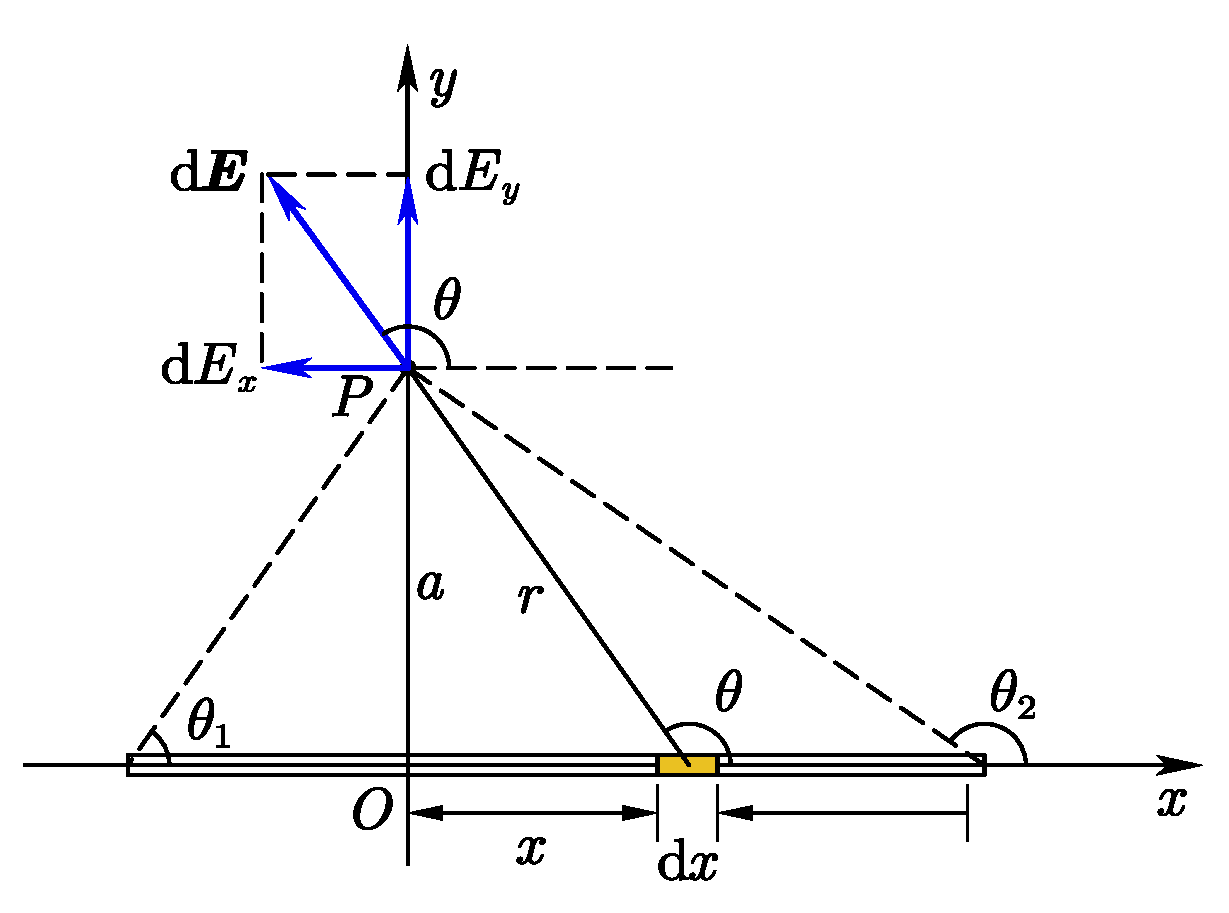
\includegraphics[width=9.5cm]{./figures/Efield_1.pdf}
\caption{均匀带电的细直棒} \label{Efield_fig1}
\end{figure}

如图,取$P$点到直棒的垂足$O$为原点,坐标轴$x$沿带电直棒,$y$通过$P$点.设直线上每单位长度所带的电荷量为$\lambda$($\lambda$就是电荷线密度),即$\lambda=q/L$. 首先在棒上离原点为$x$处取一长度为$\dd{x}$的电荷元,其电荷量为$\mathrm dq=\lambda\dd{x}$,在$P$点激发的电场强度$\mathrm d\mathbf E$为
\begin{equation}
\mathrm{d} \mathbf{E}=\frac{1}{4 \pi \varepsilon_{0}} \frac{\lambda \mathrm{d} x}{r^{2}} \mathbf e_r
\end{equation}
式中$\mathbf e_r$是从$\mathrm dx$指向$P$点的单位矢量.设$\mathrm{d} \mathbf{E}$与$x$轴之间的夹角为$\theta$,则$\mathrm{d} \mathbf{E}$沿$x$轴和$y$轴的两个分量分别为$\mathrm{d} E_{x}=\mathrm{d} E \cos \theta, \mathrm{d} E_{y}=\mathrm{d} E \sin \theta$.从图可知
\begin{equation}
x=a \tan \left(\theta-\frac{\pi}{2}\right)=-a \cot \theta, \quad \mathrm{d} x=a \csc ^{2} \theta \mathrm{d} \theta, \quad r^{2}=x^{2}+a^{2}=a^{2} \csc ^{2} \theta
\end{equation}
所以
\begin{equation}
\mathrm{d} E_{x}=\frac{\lambda}{4 \pi \varepsilon_{0} a} \cos \theta \mathrm{d} \theta, \quad \mathrm{d} E_{y}=\frac{\lambda}{4 \pi \varepsilon_{0} a} \sin \theta \mathrm{d} \theta
\end{equation}
将上列两式积分,得
\begin{equation}
\begin{aligned}E_{x}=\int \mathrm{d} E_{x}=\int_{\theta_{1}}^{\theta_{2}} \frac{\lambda}{4 \pi \varepsilon_{0} a} \cos \theta \mathrm{d} \theta=\frac{\lambda}{4 \pi \varepsilon_{0} a}\left(\sin \theta_{2}-\sin \theta_{1}\right) \\ E_{y}=\int \mathrm{d} E_{y}=\int_{\theta_{1}}^{\theta_{2}} \frac{\lambda}{4 \pi \varepsilon_{0} a} \sin \theta \mathrm{d} \theta=\frac{\lambda}{4 \pi \varepsilon_{0} a}\left(\cos \theta_{1}-\cos \theta_{2}\right)\end{aligned}
\end{equation}
电场强度的大小为
\begin{equation}
E=\sqrt{E_{x}^{2}+E_{y}^{2}}=\frac{\lambda}{4 \pi \varepsilon_{0} a} \sqrt{2-2 \cos \left(\theta_{1}-\theta_{2}\right)}
\end{equation}
其方向可用$\mathbf E$与$x$轴的夹角$\alpha$表示:
\begin{equation}
\alpha=\arctan \frac{E_{y}}{E_{x}}=\arctan \frac{\sin \theta_{2}-\sin \theta_{1}}{\cos \theta_{1}-\cos \theta_{2}}
\end{equation}
如果这一均匀带电直棒是无限长的,亦即$\theta_{1}=0, \theta_{2}=\pi$,那么
\begin{equation} \label{Efield_eq5}
E=\frac{\lambda}{2 \pi \varepsilon_{0} a}
\end{equation}
\autoref{Efield_eq5}表明,无限长带电直棒附近某点的电场强度$\mathbf E$与该点离带电直棒的距离$a$成反比,$\mathbf  E$的方向垂直于直棒.若$\lambda$为正,$\mathbf E$沿$y$轴的正方向;若$\lambda$为负,$\mathbf E$沿$y$轴的负方向.以上结果对有限长的细直棒来说,在靠近直棒中部附近的区域($a\ll L$)也近似成立.
\end{example}


\begin{example}{带电圆环的电场}\label{Efield_ex2}
\footnote{本例可类比 “球体的引力场\upref{SphF}” 中\autoref{SphF_eq2} 的推导.}在$yz$平面有一半径为$R$的圆环,均匀带有电荷量$q$. 试计算圆环轴线($x$轴)上任意一点$P$处的电场强度.
\begin{figure}[ht]
\centering
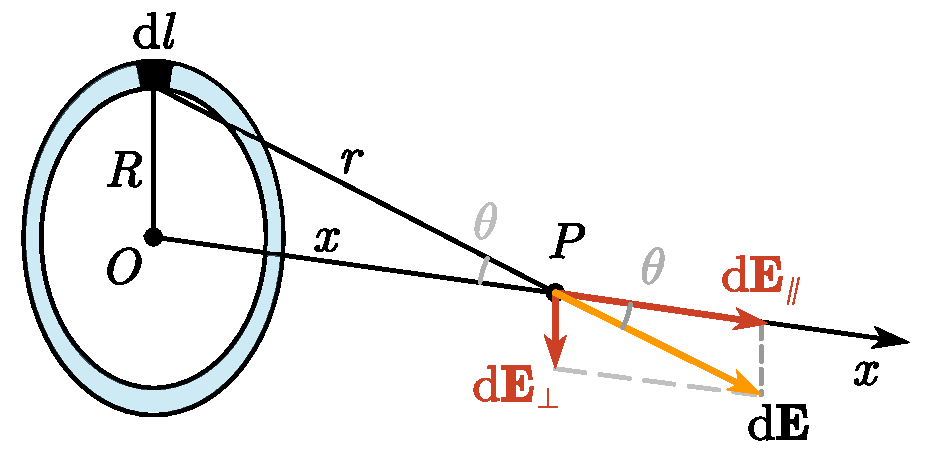
\includegraphics[width=8cm]{./figures/Efield_2.pdf}
\caption{均匀带电圆环轴线上任一点处的电场强度} \label{Efield_fig2}
\end{figure}

根据本例的轴对称性特征,将$\mathrm d\mathbf E$分解为平行于$x$轴线的分量$\mathrm d\mathbf E_\parallel$和垂直于轴线的分量$\mathrm d\mathbf E_\perp$,如\autoref{Efield_fig2}所示.

根据对称性,不难发现各电荷元的电场强度在垂直于$x$轴方向上的分矢量$\mathrm d\mathbf E$上相互抵消,所以$P$点的合电场强度是平行于$x$轴的那些分矢量$\mathrm d\mathbf E_\parallel$的总和,即
\begin{equation}
E=\int \mathrm{d} E_\parallel=\int \mathrm{d} E \cos \theta=\frac{1}{4 \pi \varepsilon_{0}} \frac{q}{2 \pi R} \frac{\cos \theta}{r^{2}} \oint \mathrm{d} l
\end{equation}
也就是
\begin{equation} \label{Efield_eq6}
E=\frac{q x}{4 \pi \varepsilon_{0}\left(x^{2}+R^{2}\right)^{3 / 2}} 
\end{equation}
若$q$为正电荷,则$\mathbf E$的方向沿$x$轴正方向;若$q$为负,则$\mathbf E$的方向沿$x$轴负方向.当$x=0$时,即在圆环中心,$E=0$;当$x\gg R$,即$P$点远离圆环时,$\left(x^{2}+R^{2}\right)^{3 / 2} \approx x^{3}$,则上式可近似地写作
\begin{equation}
E=\frac{q}{4 \pi \varepsilon_{0} x^{2}}
\end{equation}
也就是说,与环上电荷全部集中在环心处的一个点电荷所激发的电场强度相同.这点与我们的物理直觉也是相符合的.
\end{example}

 
\begin{example}{带电圆盘的电场}\label{Efield_ex3}
试计箕均匀带电圆盘轴线上与盘心$O$相距为$x$的任一给定点$P$处的电场强度.设盘的半径为$R$,电荷面密度(即单位面积上的电荷量)为$\sigma$.如\autoref{Efield_fig3}所示.

\begin{figure}[ht]
\centering
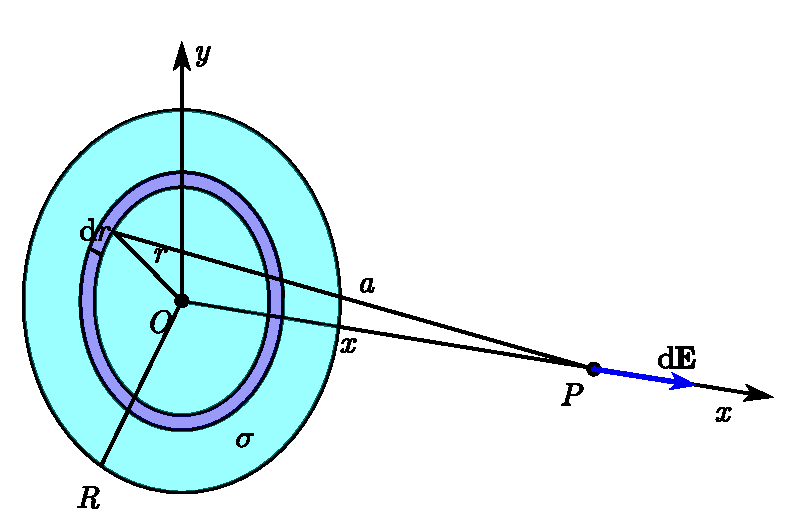
\includegraphics[width=10cm]{./figures/Efield_3.pdf}
\caption{带电圆盘的电场} \label{Efield_fig3}
\end{figure}

根据上面一个例子,很容易想到,可以把圆盘分成一系列同心的细圆环,每个细圆环可看作为电荷元,圆盘轴上各点处的电场强度就是这些半径不同的细圆环产生的电场强度的叠加.半径为$r$,宽度为$\mathrm dr$的细圆环所带的电荷量为
\begin{equation}
\mathrm{d} q=\sigma 2 \pi r \mathrm{d} r
\end{equation}
利用例题\autoref{Efield_ex2}里的结果,可得到此带电细圆环在$P$点激发的电场强度为
\begin{equation}
\mathrm{d} E=\frac{x \mathrm{d} q}{4 \pi \varepsilon_{0}\left(x^{2}+r^{2}\right)^{3 / 2}}=\frac{1}{4 \pi \varepsilon_{0}} \frac{x}{\left(x^{2}+r^{2}\right)^{3 / 2}} \sigma 2 \pi r \mathrm{d} r=\frac{\sigma x}{2 \varepsilon_{0}} \frac{r \mathrm{d} r}{\left(x^{2}+r^{2}\right)^{3 / 2}}
\end{equation}
由于各带电细圆环在$P$点激发的电场强度的方向都相同,而带电圆盘的电场强度就是这些带电细圆环所激发的电场强度的矢量和,所以
\begin{equation}\label{Efield_eq7}
E=\int \mathrm{d} E=\frac{\sigma x}{2 \varepsilon_{0}} \int_{0}^{R} \frac{r \mathrm{d} r}{\left(x^{2}+r^{2}\right)^{3 / 2}}=\frac{\sigma}{2 \varepsilon_{0}}\left(1-\frac{x}{\sqrt{R^{2}+x^{2}}}\right)
\end{equation}
电场强度$\mathbf E$的方向与圆盘相垂直,其指向则视$\sigma$的正负而定.$\sigma>0$,则$\mathbf E$沿$x$轴正方向;$\sigma<0$,则$\mathbf E$沿$x$轴负方向.

我们来看两个特殊情况.

若$R\gg x$,即在$P$点看来可认为均匀带电圆盘为\textbf{无限大},则$P$点的电场强度可由对上式取极限求得:
\begin{equation} \label{Efield_eq8}
E=\frac{\sigma}{2 \varepsilon_{0}}
\end{equation}
只要$P$点与任意带电平面间的距离远小于该点到带电平面边缘各点的距离,即对均匀带电平面中部附近各点来说,这平面都可看作是无限大,其电场强度都可以由\autoref{Efield_eq8}近似表示.这表明无限大均匀带电平面所激发的电场与距离$x$无关,在平面两侧各点有大小相等、方向都与平面相垂直的\textbf{匀强电场}或称作\textbf{均匀电场(uniform electric field)}.

若$x\gg R$,利用二项式定理展开的近似式,略去$R/x$的高次项后可以把\autoref{Efield_eq7}的括号中后一项处理为
\begin{equation}
\left(1+\frac{R^{2}}{x^{2}}\right)^{-1 / 2}=1-\frac{1}{2} \frac{R^{2}}{x^{2}}+\frac{3}{8}\left(\frac{R^{2}}{x^{2}}\right)^{2}-\cdots \approx 1-\frac{1}{2} \frac{R^{2}}{x^{2}}
\end{equation}
于是$P$点的电场强度大小为
\begin{equation}
E=\frac{\sigma R^{2}}{4 \varepsilon_{0} x^{2}} =\frac{q}{4 \pi \varepsilon_{0} x^{2}} 
\end{equation}

式中$q=\sigma\pi r^2$是圆盘所带电荷量.由此可见,当$P$点离开圆盘的距离比圆盘本身的大小大得多时,$ P$点的电场强度与电荷量$q$集中在圆盘的中心的一个点电荷在该点所激发的电场强度相同.
\end{example}
